\documentclass[aspectratio=1610]{beamer}
\usefonttheme{professionalfonts}
\usetheme{metropolis}
\setbeamertemplate{bibliography item}{\insertbiblabel}
\usepackage{polyglossia}
\setmainlanguage{english}
\usepackage{amsmath}
\usepackage{amssymb}
\usepackage{mathtools}
\usepackage{graphicx}
\usepackage[version=4]{mhchem}
\usepackage[
  math-style=ISO,
  bold-style=ISO,
  sans-style=italic,
  nabla=upright,
]{unicode-math}
\setmathfont{Latin Modern Math}
\usepackage{blindtext}
\usepackage{fontspec}
\title{}
\subtitle{}
\date{\today}
\author{Steven Becker}
\usepackage{siunitx}
\AtBeginDocument{
\sisetup{
math-rm=\mathrm,
math-micro=μ,
}
}
\usepackage{framed}
\usepackage{biblatex}
\addbibresource{lit.bib}
\usepackage{booktabs}

\begin{document}

\frame{\maketitle}


%\begin{frame}
%\tableofcontents
%\end{frame}


\begin{frame}{ Überblick }
  \begin{itemize}
    \setlength\itemsep{1.2em}
      \item{ Situation in Deutschland }
      \item{ Weg zum Rückbau }
      \item{ Der Rückbau }
      \item{ Kosten }
  \end{itemize}
\end{frame}






\begin{frame}{ Situation in Deutschland }
  \begin{columns}

    \begin{column}{0.48\textwidth}
      \begin{figure}
        \centering
        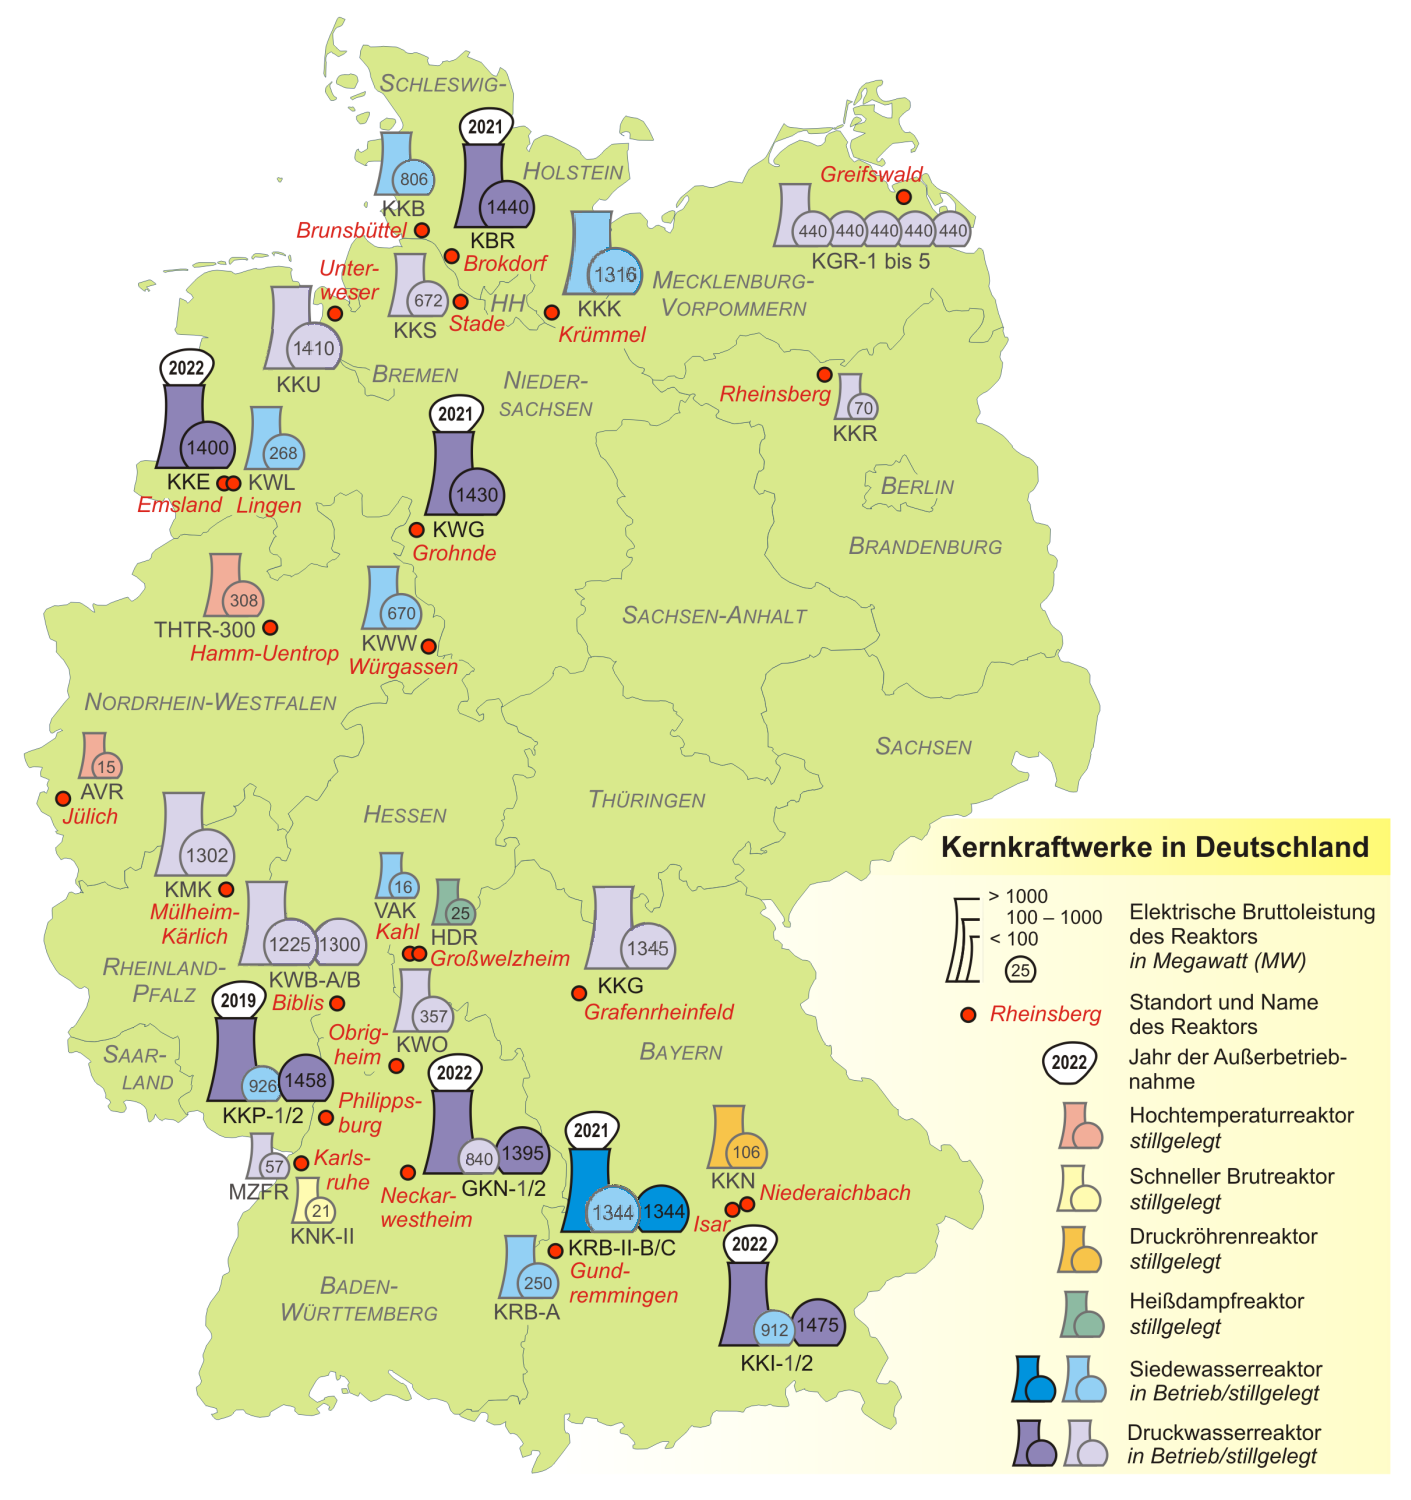
\includegraphics[width=1\textwidth]{./bilder/Kernkraftwerke_in_Deutschland.png}
        \caption{ Auflistung aller deutschen Akws \cite{karte_abschaltungen}. }
        \label{ fig: karte_abschaltungen }
      \end{figure}
    \end{column}

    \begin{column}{0.48\textwidth}
      \begin{itemize}
        \setlength\itemsep{1.2em}
          \item{ 27 Akws mit 36 Reaktoren }
          \item{ 38 Forschungsreaktoren}
          \item{ 2022 letzte Abschaltung }
        \end{itemize}
    \end{column}
  \end{columns}
\end{frame}



\section{Weg zum Rückbau}



\begin{frame}{ Stillegung }
   \begin{columns}

    \begin{column}{0.48\textwidth}
      \begin{itemize}
       \setlength\itemsep{1.2em}
         \item{ Stillegungen müssen beantragt werden}
         \item{ Zuständigkeitsbereich der Länder}
         \item{ Unterliegt dem Atomrecht}
         \item{ 2 Stillegungsstrategien \\ Direkter Abbau und Sicher Einschluss}
      \end{itemize}
    \end{column}

    \begin{column}{0.48\textwidth}
      \begin{figure}
        \centering
        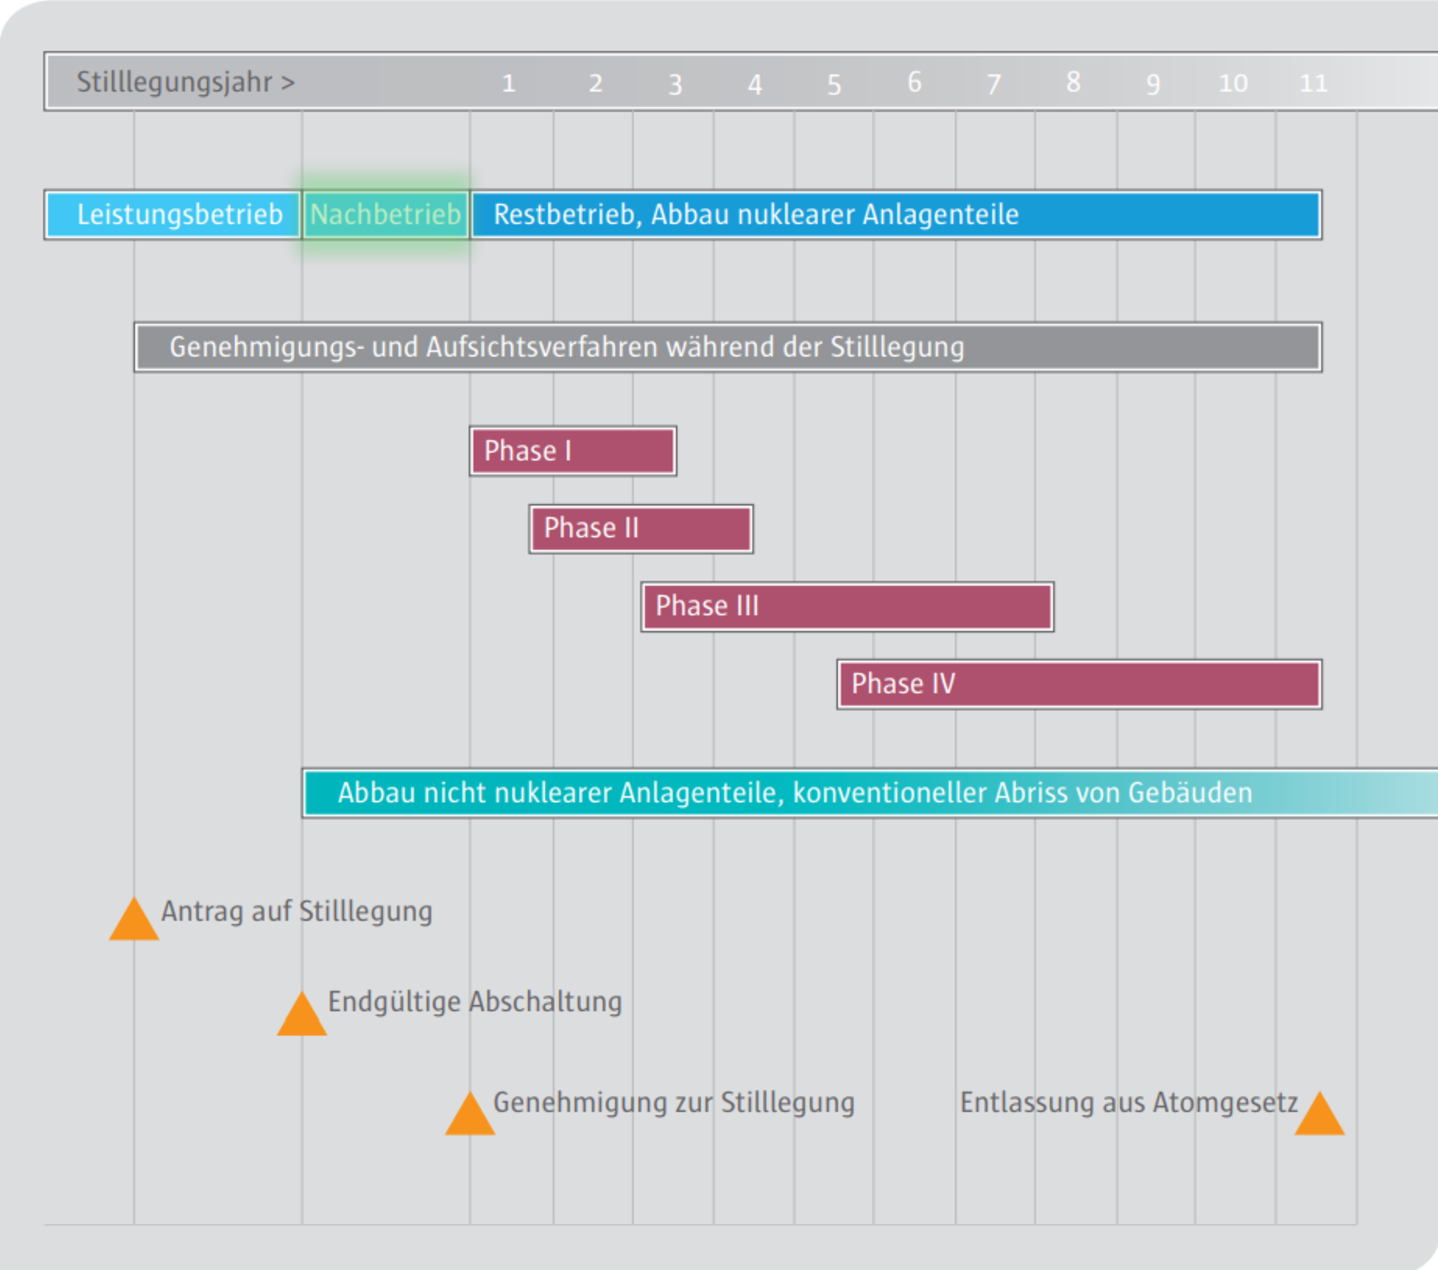
\includegraphics[width=1.05\textwidth]{./bilder/stilllegung_nachbetrieb.pdf}
        \caption{ Zeitlicher Verlauf eines direkten Abbau\cite{stilllegung_grs}. }
        \label{ fig: stillegung }
      \end{figure}
    \end{column}

  \end{columns}
\end{frame}



\begin{frame}{ Nachbetriebsphase }
  \begin{columns}

    \begin{column}{0.48\textwidth}

        \begin{itemize}
          \setlength\itemsep{1.2em}
          \item{ Abschaltung des Kernreaktors }
          \item{ Dauer von etwa 5 Jahren nach der Abschlatung}
          \item{ Brennelemente müssen eine Zeit lang weiter gekühlt werden }
          \item{ radioaktive Betriebsabfälle werden entfernt }
        \end{itemize}

    \end{column}

    \begin{column}{0.48\textwidth}
      Senkung der durchschnitllichen Aktivität
      \begin{equation*}
        \SI{10e20}{\becquerel} \quad \rightarrow  \quad \SI{10e16}{\becquerel}
      \end{equation*}
    \end{column}

  \end{columns}
\end{frame}



\begin{frame}{Stillegungstrategien - Sicherer Einschluss}
  \begin{itemize}
    \setlength\itemsep{1.2em}
    \item{ Nach der Abschaltung wird der Reaktor in eine wartungsarmen Zustand gebracht} 
    \item{ Kontrollbereich wird versiegelt}
    \item{ Regelmäßige Kontrollen nötig}
    \item{ Einschlusszeit von ca. $30$ Jahren}
  \end{itemize}
\end{frame}



\begin{frame}{Stillegungstrategien - Direkter Abbau}
   \begin{itemize}
    \setlength\itemsep{1.2em}
      \item{ Rückkbau unmittelbar nach Abschaltung }
      \item{ Know-How der Miterbeiter bleibt erhalten}
      \item{ In Deutschland am häufigstens verwendet}
  \end{itemize}
\end{frame}



\begin{frame}{ Direkter Abbau - Sicherer Einschluss - Ein Vergleich}
  \begin{figure}
     \centering
     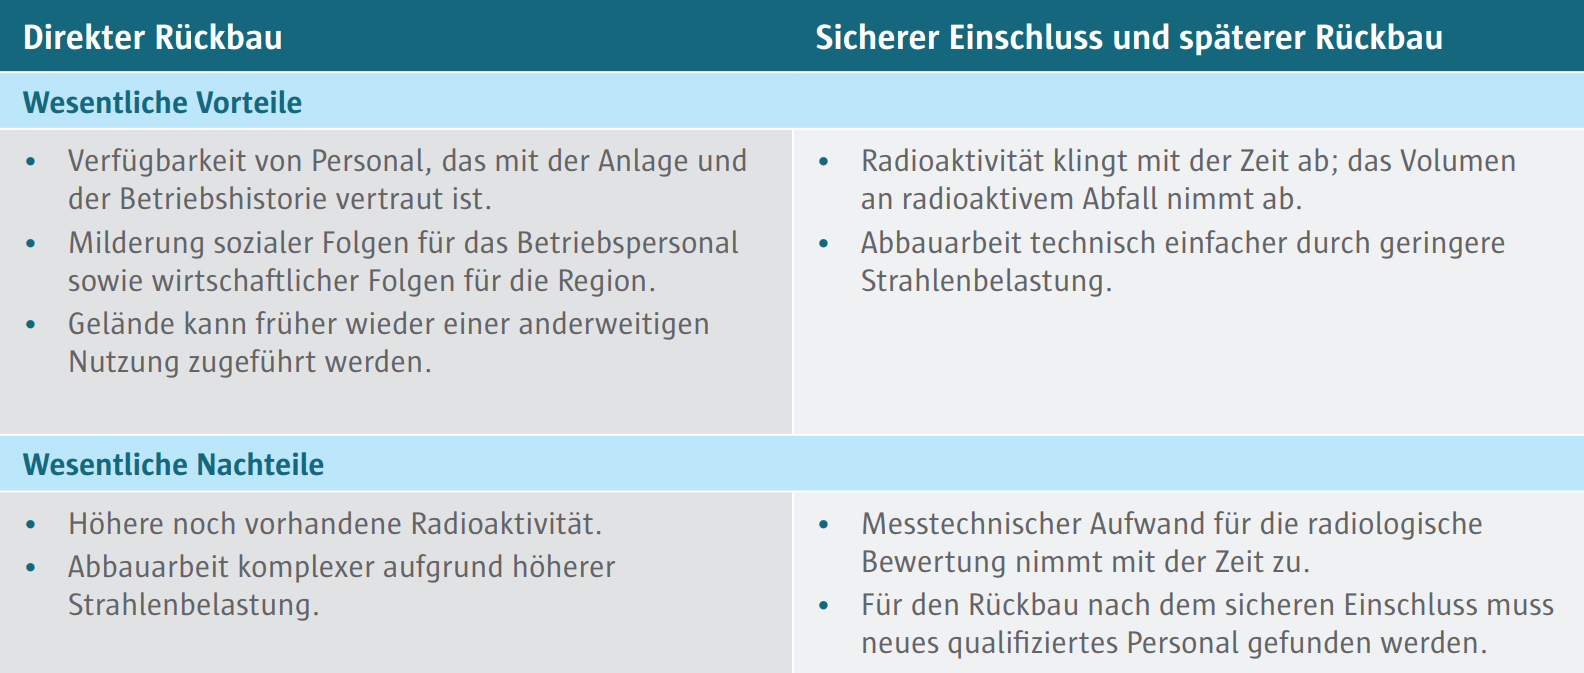
\includegraphics[width=1\textwidth]{./bilder/vor_nachteile_direkter_einschluss.PNG}
     \caption{ Vor- und Nachteile von Direkter Abbau und Sicheren Einschluss \cite{stilllegung_grs}. }
     \label{ fig: karte_abschaltungen }
   \end{figure}
\end{frame}



\begin{frame}
  \begin{columns}
  
      \begin{column}{0.2\textwidth}
        \section{Der Rückbau}
      \end{column}
  
      \begin{column}{0.78\textwidth}
        \begin{figure}
          \centering
          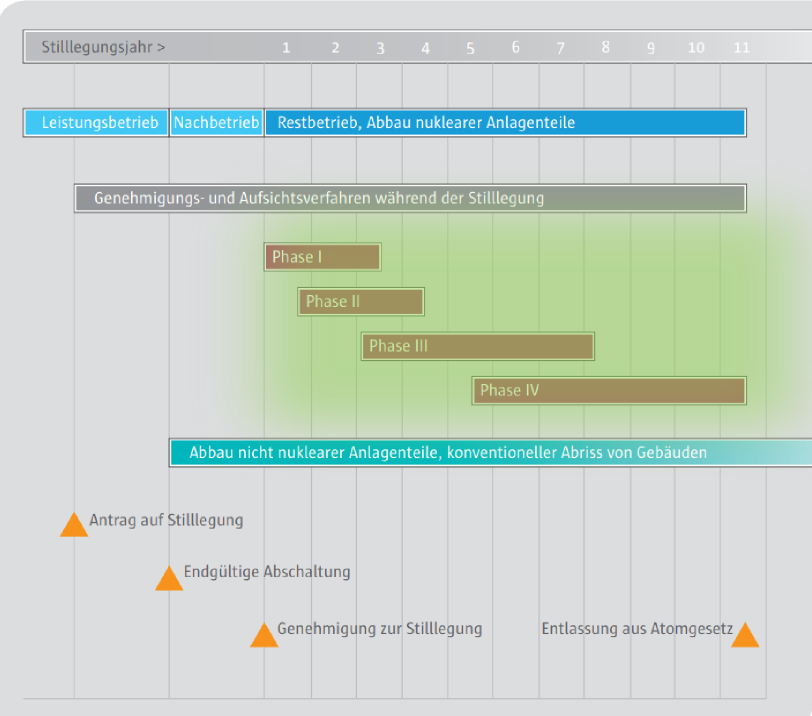
\includegraphics[width=0.8\textwidth]{./bilder/stillegung_phasen.png}
          \caption{ Zeitlicher Verlauf eines direkten Abbau\cite{stilllegung_grs}. }
          \label{ fig: stillegung }
        \end{figure}
      \end{column}

  \end{columns}
\end{frame}



\begin{frame}{Phase 1}
  \begin{columns}

    \begin{column}{0.48\textwidth}
      \begin{itemize}
        \setlength\itemsep{1.2em}
        \item{ Ausbau von nicht mehr benötigten Teilen z.\, B. Regelstabführungen }
        \item{ Platz schaffen für spätere Rückbaumaßnahmen}
        \item{ Rückbauarbeiten im Maschinenhaus}
      \end{itemize}
    \end{column}

    \begin{column}{0.48\textwidth}
      \begin{figure}
         \centering
         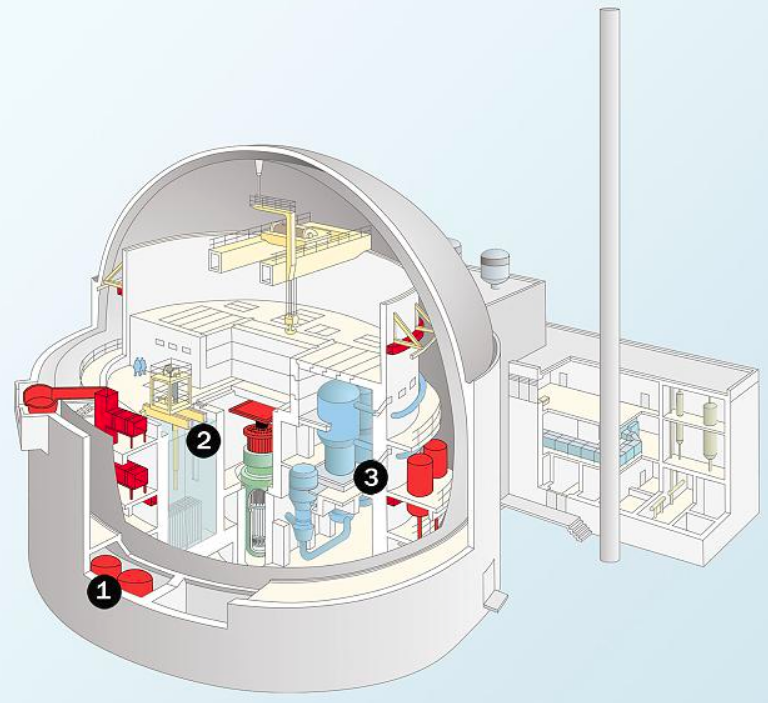
\includegraphics[width=0.85\textwidth]{./bilder/abbau_phase_1_spiegel.png}
         \caption{Schematische Darstellung der Bauteile die von der Rückbauphase 1 betroffen sind und ausgebaut werden, am Beispiel eines Druckwasserreaktors \cite{abbau_grafik_stade}. }
         \label{ fig: phase_1 }
       \end{figure}
    \end{column}

  \end{columns}
\end{frame}



\begin{frame}{Phase 2}
  \begin{columns}

    \begin{column}{0.48\textwidth}
      \begin{figure}
         \centering
         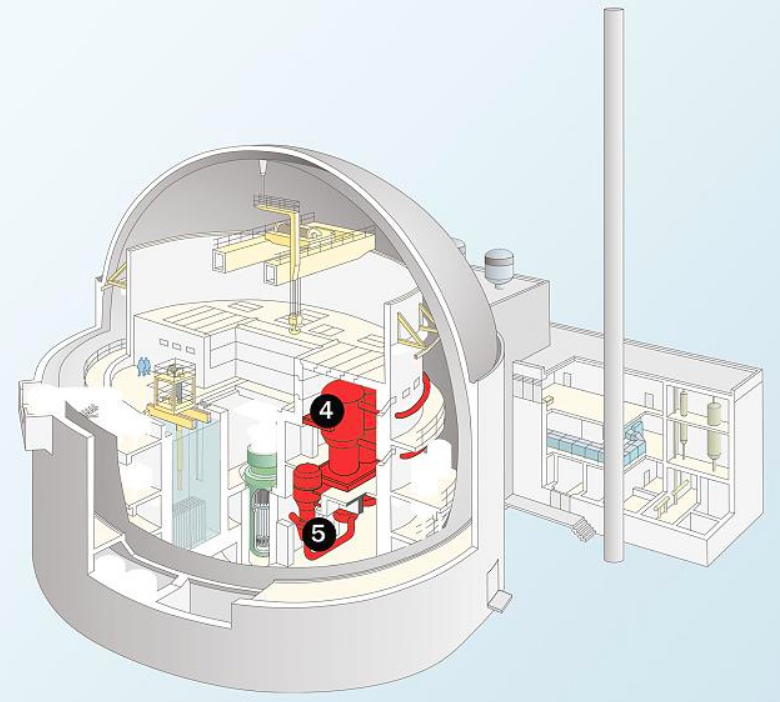
\includegraphics[width=0.85\textwidth]{./bilder/abbau_phase_2_spiegel.png}
         \caption{ Schematische Darstellung der Bauteile die von der Rückbauphase 2 betroffen sind und ausgebaut werden, am Beispiel eines Druckwasserreaktors \cite{abbau_grafik_stade}. }
         \label{ fig: phase_2 }
       \end{figure}
     \end{column}

     \begin{column}{0.48\textwidth}
       \begin{itemize}
         \setlength\itemsep{1.2em}
        \item{ Dauer von etwa 2 Jahren}
         \item{ Entfernung des Kühlkreislaufes }
         \item{ Abbau des Dampferzeugers}
       \end{itemize}
     \end{column}

  \end{columns}
\end{frame}



\begin{frame}{Phase 3}
  \begin{columns}

    \begin{column}{0.48\textwidth}
      \begin{figure}
         \centering
         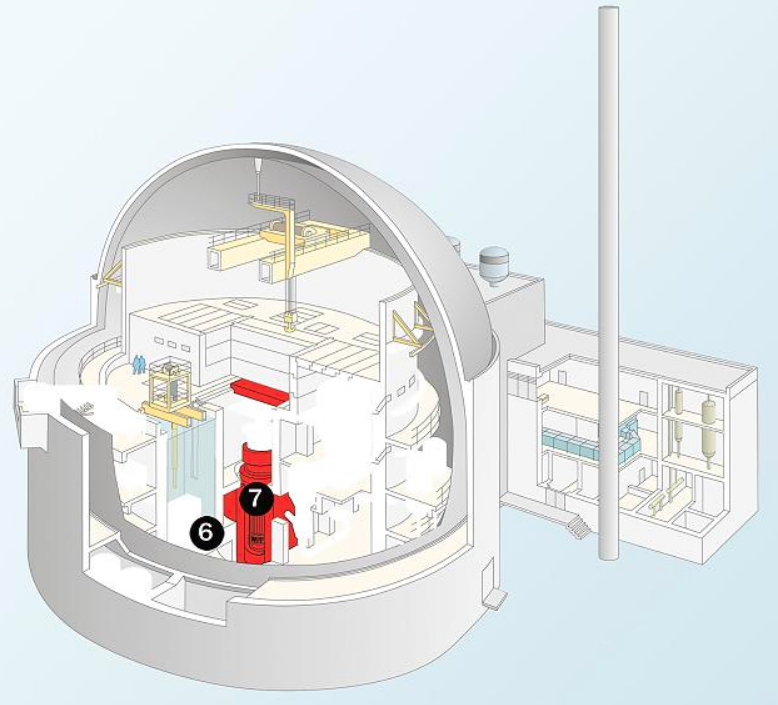
\includegraphics[width=0.85\textwidth]{./bilder/abbau_phase_3_spiegel.png}
         \caption{Schematische Darstellung der Bauteile die von der Rückbauphase 3 betroffen sind und ausgebaut werden, am Beispiel eines Druckwasserreaktors \cite{abbau_grafik_stade}. }
         \label{ fig: phase_3 }
       \end{figure}
     \end{column}

     \begin{column}{0.48\textwidth}
       \begin{itemize}
         \setlength\itemsep{1.2em}
         \item{ Dauer von etwa 3 Jahren}
         \item{ Entfernung des Reaktordruckbehälters }
         \item{ Rückbau des biologischen Schildes }
       \end{itemize}
     \end{column}

  \end{columns}
\end{frame}



\begin{frame}{Phase 4}
  \begin{columns}

    \begin{column}{0.48\textwidth}
      \begin{itemize}
        \setlength\itemsep{1.2em}
        \item{ Abwassseraufbereitung und Abluftanlage werden entfernt}
        \item{ Gebäudekontamination }
        \item{ Atomrechtliche Überwachung endet}
      \end{itemize}
    \end{column}

    \begin{column}{0.48\textwidth}
      \begin{figure}
         \centering
         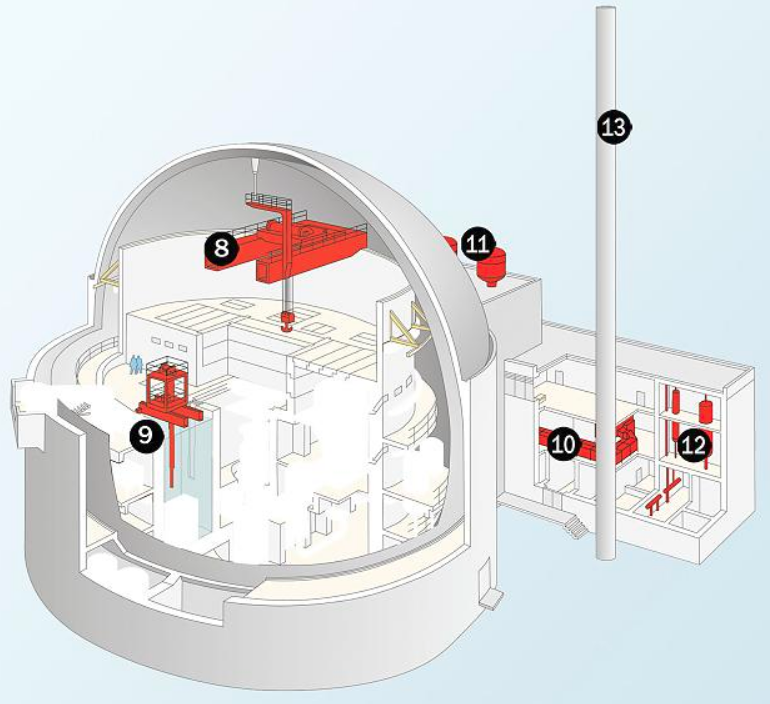
\includegraphics[width=0.85\textwidth]{./bilder/abbau_phase_4_spiegel.png}
         \caption{Schematische Darstellung der Bauteile die von der Rückbauphase 4 betroffen sind und ausgebaut werden, am Beispiel eines Druckwasserreaktors \cite{abbau_grafik_stade}. }
         \label{ fig: phase_4 }
       \end{figure}
    \end{column}

  \end{columns}
\end{frame}



\begin{frame}{Demontierungsverfahren}
  \begin{columns}

    \begin{column}{0.48\textwidth}
    \begin{itemize}
      \setlength\itemsep{1.2em}
      \item{Strahlenexpositionen für das Personal müssen möglichst gering sein }
      \item{ räumliche Randbedinungen }
      \item{ Verwendung von mechanische und thermische Verfahren }

    \end{itemize}

    \end{column}

    \begin{column}{0.48\textwidth}
      \begin{figure}
         \centering
         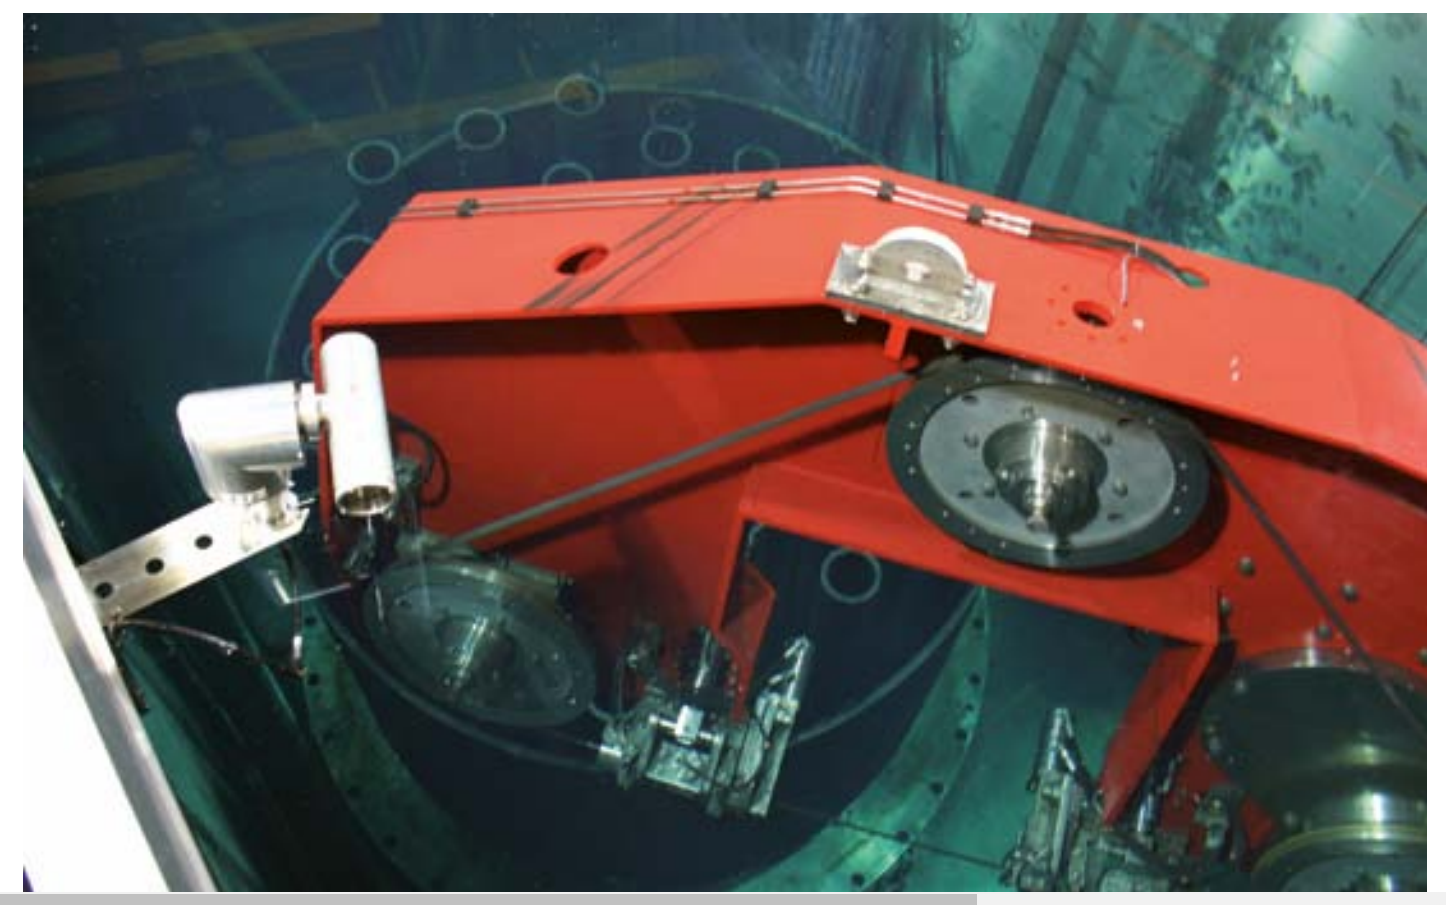
\includegraphics[width=0.95\textwidth]{./bilder/zerlegung_bandsaege.PNG}
         \caption{Zerlegung des Reaktordruckbehälters unter Wasser mit einer ferngesteuerten Bandsäge \cite{stilllegung_grs}. }
         \label{ fig: abbau_roboter}
       \end{figure}
    \end{column}

  \end{columns}
\end{frame}



\begin{frame}{Radioaktiver Abfall -Neutronaktivierung}
  \begin{columns}

    \begin{column}{0.48\textwidth}
      \begin{itemize}
        \setlength\itemsep{1.2em}
        \item{Brennelemente}
        \item{z.\,B. Kühlmittel, Beton und Stahl auf Grund von Neutroneneinfang}
        \item{ Vergößerung der Menge an radioaktove Abfall}
      \end{itemize}
    \end{column}

    \begin{column}{0.48\textwidth}
        \begin{figure}
           \centering
           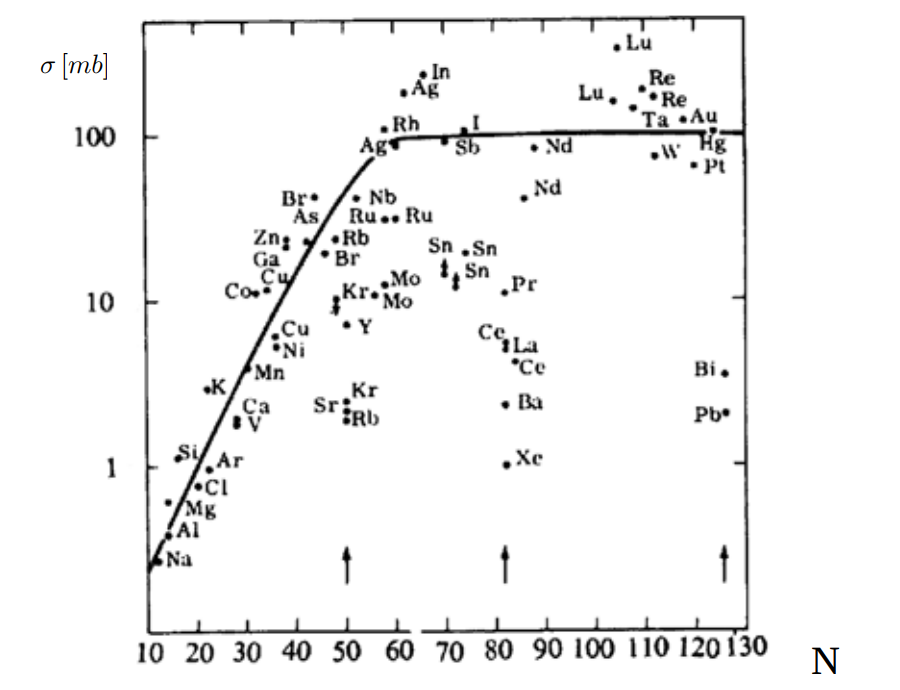
\includegraphics[width=1.05  \textwidth]{./bilder/einfangwahrscheinlichkeit_neutron.png}
           \caption{Einfangsquerschnitt fur Neutronen als Funktion der Neutronenzahl der Kerne \cite{neutroneneinfang}. }
           \label{ fig: abbau_roboter}
         \end{figure}
    \end{column}

  \end{columns}
\end{frame}



\begin{frame}{Neutronaktivierung}
  \begin{align*}
    \shortintertext{Stahl}
    ^{58}_{26}\ce{Fe}+ ^1_0\mathrm{n }\quad &\rightarrow \quad  ^{59}_{26}\ce{Co} \quad \rightarrow \quad ^{59}_{27}\ce{Fe} + _{-1}^{0}\ce{e}+\gamma \\
  \shortintertext{Beton}
    ^{44}_{20}\ce{Ca}+ ^1_0\mathrm{n }\quad &\rightarrow \quad  ^{45}_{20}\ce{Ca} \quad \rightarrow \quad ^{45}_{21}\ce{Sc} + _{-1}^{0}\ce{e}+\gamma
  \end{align*}
\end{frame}




\begin{frame}{Radioaktiver Abfall}
  \begin{figure}
     \centering
     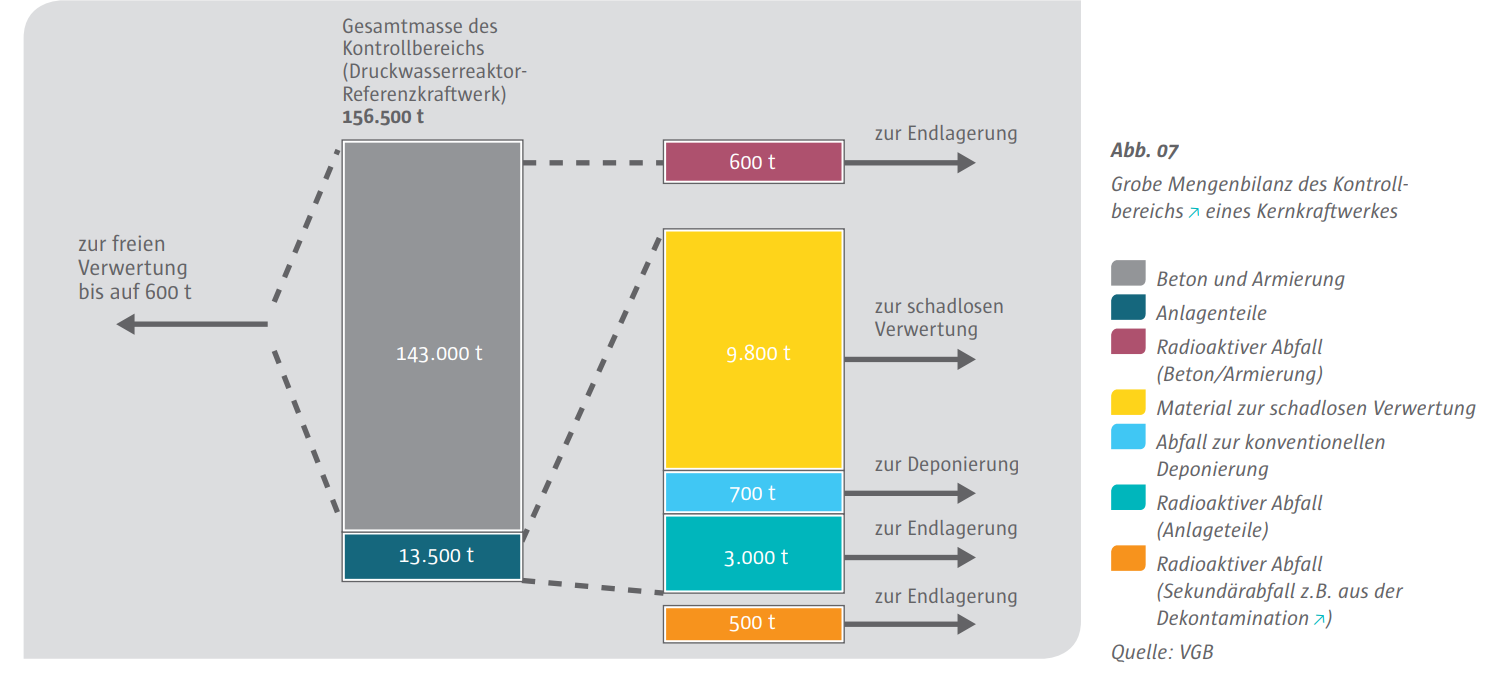
\includegraphics[width=0.95\textwidth]{./bilder/radioakives_material.PNG}
     \caption{Gesamtmaterial im Kontrollbereiches \cite{muell}. }
     \label{ fig: muell_kontrollbereich}
   \end{figure}
\end{frame}



\begin{frame}{Dekontamination}
  \begin{itemize}
    \setlength\itemsep{1.2em}
    \item{ Verrinerrung der Radioaktivität}
    \item{ Aktivierung am stäkrsten an der Oberfläche}
    \item{ Verwendung von mechanischen und chemischen Verfahren}
    \item { Reinigung der Oberfläche oder Entfernen der obersten Schicht}
  \end{itemize}
\end{frame}

\begin{frame}{Gebäudedekontamination}
  \begin{columns}

    \begin{column}{0.48\textwidth}
      \begin{itemize}
        \setlength\itemsep{1.2em}
        \item{ mittels Shaver die Wandbeschichtungen abgetragen (vgl. Abb. \ref{fig: gebaeudekontamination})}
        \item {Bagger entfernen kontaminierte Betonstrukturen }
      \end{itemize}
    \end{column}

    \begin{column}{0.48\textwidth}
      \begin{figure}
         \centering
         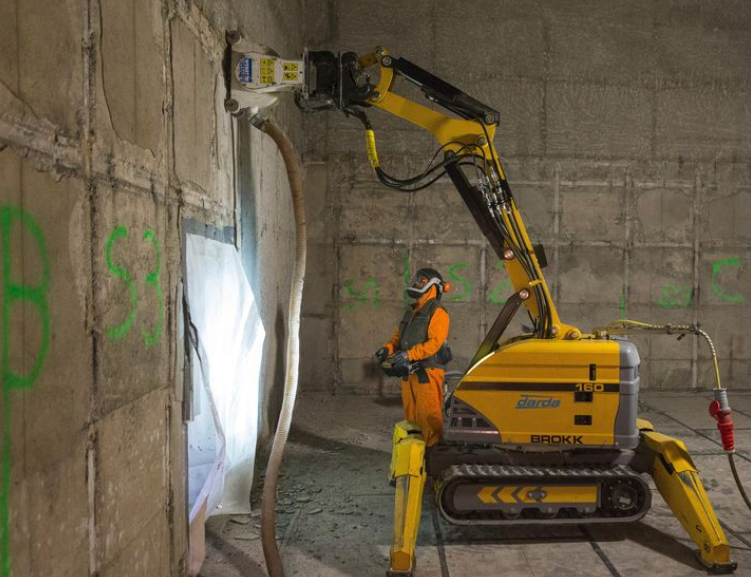
\includegraphics[width=1\textwidth]{./bilder/gebaeudedekontamination.png}
         \caption{Gebäudekontamination im Kernkraftwerk Greifswald mit Hilfe von Shaver \cite{gebauededekontamination}. }
         \label{fig: gebaeudekontamination}
       \end{figure}
    \end{column}

  \end{columns}
\end{frame}


\begin{frame}{Freigabe}
  \begin{columns}

    \begin{column}{0.48\textwidth}
      \begin{figure}
         \centering
         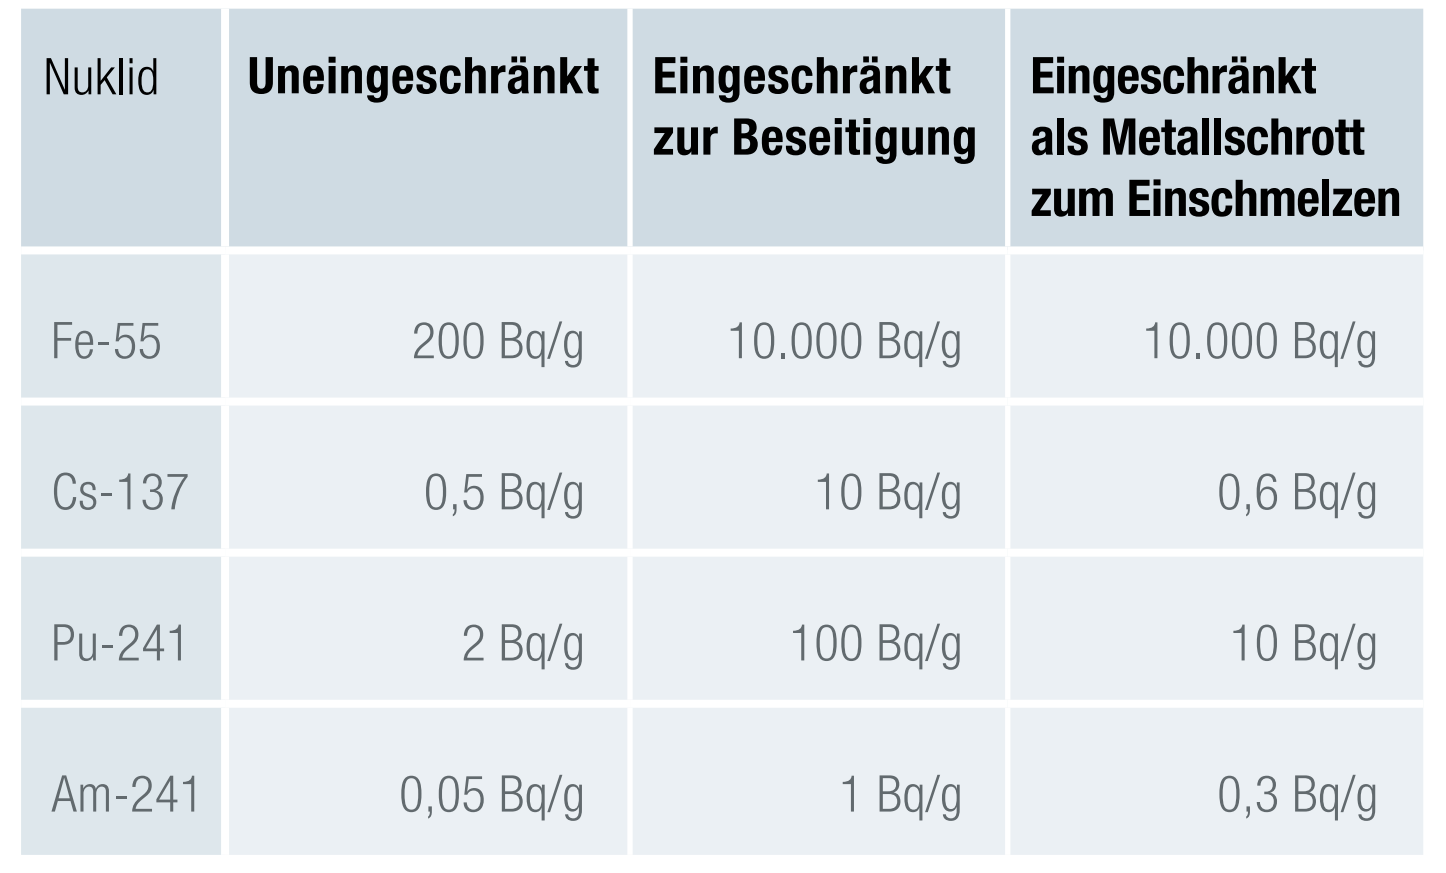
\includegraphics[width=1\textwidth]{./bilder/freigabeoption.PNG}
         \caption{Freigabegrenzwerte für verschiedene Nuklide \cite{stilllegung_grs}. }
         \label{ fig: freigabegrenzwerte}
       \end{figure}
    \end{column}

    \begin{column}{0.48\textwidth}
      \begin{itemize}
        \setlength\itemsep{1.2em}
        \item{ sinkt die Aktivität eines Materials unter ein bestimmtes Niveau, kann es freigegeben werden }
        \item{ Muss für jedes Teil einzeln entschieden werden}
        \item {Es gibt verschiedene Freigabestufen}
      \end{itemize}
    \end{column}

  \end{columns}
\end{frame}



\section{Kosten}



\begin{frame}{Kosten}
  \begin{itemize}
    \setlength\itemsep{1.2em}
    \item{ Betreiber bauen Rückstellungen auf, von denen der Rückbau bezahlt werden soll}
    \item{ 2014 beliefen sich die Rückstellungen auf $\num{37.6} \, \mathrm{Mrd} \,\euro$}
    \item{Kosten für den Rückbau der Kraftwerke in Deutschland wird auf  $\num{47.5} \, \mathrm{Mrd} \,\euro$ geschätzt}
  \end{itemize}
\end{frame}



\begin{frame}{Zusammenfasssung}
  \begin{itemize}
    \setlength\itemsep{1.2em}
    \item { Es exestieren zwei Rückbaustrategien:  Direkter Abbau  Sicherer Einschluss}
    \item { Rückbau läuft in vier Phasen ab }
    \item { Material wird Dekontaminiert}
    \item { Rückbau der Kraftwerke in Deutschland wird auf  $\num{47.5} \, \mathrm{Mrd} \,\euro$ geschätzt}
  \end{itemize}
\end{frame}

\begin{frame}[allowframebreaks]
  \nocite{*}
  \printbibliography
\end{frame}

\end{document}
